
\begin{figure}[h]
    \centering
    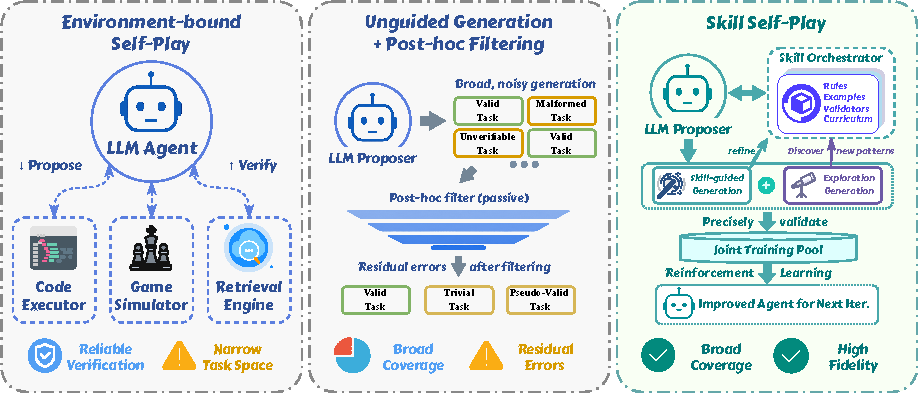
\includegraphics[width=0.98\linewidth]{figures/intro.pdf} 
    
    \caption{{Motivation of \textbf{Skill Self-play}.}
    \textbf{Left:} \emph{Environment-bound methods} provide reliable verification but severely restrict the task space.
    \textbf{Middle:} \emph{Unguided generation} broadens coverage but depends on passive post-hoc filtering, allowing residual errors to degrade data fidelity.
    \textbf{Right:} \emph{Skill Self-Play} uses a proactive Skill Orchestrator with dual streams for skill-guided generation and open-ended exploration, enabling iterative skill evolution with both broad coverage and high fidelity.}

    \label{fig:intro}
\end{figure}


\section{Introduction}
\label{sec:introduction}


\begin{wrapfigure}{r}{0.39\textwidth}
    \vspace{-1.5em}
    \centering
    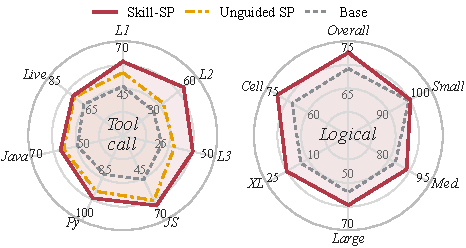
\includegraphics[width=\linewidth]{figures/fig_qwen3_4b_performance_radar.pdf}
    \vspace{-1.8em}
    \caption{\textbf{Performance footprint.} Skill-SP broadly expands Qwen3-4B-Ins capabilities across tool-calling and logical reasoning. Notably, Unguided SP is absent from the latter as it fails to synthesize valid puzzles.}
    \vspace{-1.0em}
    \label{fig:intro_radar}
\end{wrapfigure}



Self-evolution methods, which empower Large Language Models (LLMs) to autonomously generate tasks, find solutions, and evaluate outcomes, have shifted the post-training paradigm from heavy data-driven annotation to self-improvement without any supervision~\citep{tao2024survey,patel2024large,jiang2024long,chen2025multi,xu2025genius}. Along this new scaling dimension, self-play has emerged as a foundational technique, in which the learning LLM engages in gameplay as different role-playing agents and updates its policies via multi-agent reinforcement learning (MARL)~\citep{yang2025spell,yuan2025marshal,liu2025spiral,jiang2026one}. Recent works have demonstrated the surprising power of self-play across various scenarios, significantly boosting LLM capabilities in domains such as logical reasoning~\citep{cheng2024self,huang2025r}, deep search~\citep{lu2025search,liu2025spice}, visual question answering~\citep{wang2025vision}, and software engineering~\citep{wei2025toward,zhao2026absolute}.




However, the success of self-play in each specific domain depends heavily on well-crafted environments and rewards to provide precise validation~\citep{yang2026self,song2026envscaler,yan2026openskill,huang2026ace,wang2026code}. 
While external verification ensures accuracy, it confines agent training to narrow operational boundaries, leaving the model unable to generalize to broader, open-ended tasks~\citep{tang2025beyond,zhao2025learning}. 
To broaden the task space, alternative approaches employ unguided task generation paired with post-hoc filtering (e.g., format checks or majority voting)~\citep{wang2023self,xu2024wizardlm,nguyen2024better,xu2025magpie,an2025ultraif,yu2025cot}. 
Unfortunately, open-ended task generation severely compromises quality control~\citep{long2024llms,jiang2025self}. 
Without structural guidance, task generators frequently synthesize ill-posed tasks or overfit to simple templates~\citep{yu2025guided,li2026r}.
Over successive training iterations, accumulated errors and biases cause synthetic data collapse~\citep{shumailov2024ai,kazdan2025collapse}.
Ultimately, post-hoc filtering acts merely as a \emph{passive sieve}: it rejects glaring formatting errors but cannot actively guide the generator to produce reusable, logically valid, and diverse task patterns. 
Consequently, a fundamental challenge remains: \emph{How can self-play autonomously generate and verify diverse agent tasks without collapsing into either narrow domains or chaotic synthetic noise?}



To resolve this dilemma and bridge the gap between rigid environments and passive filtering~\citep{khattab2023dspy,dong2025self,prabhakar2026apigen,gao2026self}, we argue that verifiable self-play can be significantly enhanced by the concept of \emph{skills}. 
As introduced by~\citet{claudeIntroducingAgent}, a skill is a modular unit of procedural knowledge that bundles task-specific instructions and supporting resources into a reusable block. By organizing expertise into these self-contained units, skills allow agents to dynamically load specialized knowledge exactly when needed.
When formalized as a \emph{task-pattern interface}, this proactive abstraction serves as the ideal medium of evolution. 
While raw execution rollouts in self-play contain valuable insights, this evolutionary knowledge is typically scattered across isolated trajectories. 
Simply aggregating these experiences by stuffing historical trajectories into a single task-generator prompt leads to severe context bloat and dilutes structural control. 
In contrast, a skill interface distills this scattered experience into a compact, reusable, and co-evolvable unit. 
Rather than acting as a passive post-hoc filter, this interface actively orchestrates the entire self-play loop: injecting structural priors to guide the task generator \emph{before} synthesis, providing explicit executable mechanisms for rigorous verification \emph{after} response generation, and tracking historical difficulty to govern curriculum progression \emph{across} successive iterations.




To realize this paradigm, we introduce \emph{\textbf{Skill} \textbf{S}elf-\textbf{P}lay} (\textbf{Skill-SP}), a reinforcement learning framework driven by an evolving library of modular skill packages (Figure~\ref{fig:intro}). 
At its core, Skill-SP orchestrates self-play through three core components: a \emph{Proposer}, a \emph{Solver}, and a \emph{Controller}. 
More specifically, the Proposer synthesizes targeted challenges guided by routed skill packages; the Solver learns to execute and solve these tasks; and the Controller analyzes execution trajectories to continually manage the skill library. 
Within this loop, the skill library undergoes a continuous evolutionary cycle: the Controller automatically refines existing skill packages based on execution feedback, archives obsolete ones, and induces entirely new skills from open-ended exploration. 
This dynamic routing of modular skills ensures strict structural quality control without context bloat, while the discovery of new skill packages continuously expands the task frontier. 
By isolating governance in this evolving library, Skill-SP successfully resolves the fundamental tension between task diversity and verification reliability.
%
%
We empirically validate Skill-SP on two families of verifiable agent tasks: tool calling (API-Bank~\citep{li2023api} and BFCL~\citep{patil2025berkeley}) and logical reasoning (ZebraLogic~\citep{lin2025zebralogic}). Across various open-source LLM backbones, Skill-SP delivers substantial performance breakthroughs, yielding absolute gains of up to \textbf{+42.9} points on tool use and \textbf{+12.0} points on logical reasoning, consistently outperforming unguided self-play (as in Figure~\ref{fig:intro_radar}).
Finally, diagnostic analyses confirm that Skill-SP successfully anchors task generation at the model's evolving learning frontier by continuously distilling novel patterns into reusable skills. The proposed skill-driven self-play brings a fundamental paradigm shift to model self-improvement, unlocking a sustainable and truly open-ended frontier for LLM self-evolution.